% !TEX root = ../main.tex

\chapter{Experiments}
\label{ch:experiments}
The goal of this chapter is to answer the research questions formulated in Section~\ref{sec:research_questions}. First, I describe which experiments I conducted. Next, I show the results of the experiments. Finally, I discuss the results further in the last section.

\section{Experiments}
This section describes the experiments I used in order to investigate and answer the formulated research questions. We can break down the experiments into three categories: reproduction of the results of the paper \emph{Analyzing Reinforcement Learning Benchmarks with Random Weight Guessing}, comparison of the alternative models described in Section~\ref{sec:models} to neural networks, and an analysis of the impact of bias.

\subsection{Reproduction of RWG-Paper}
For a starting point, I reproduced the results of the paper \emph{Analyzing Reinforcement Learning Benchmarks with Random Weight Guessing} discussed in Section~\ref{sec:benchmarks}. I used the same methodology as the authors of the paper did. In specific, I used three network architectures: a network without any hidden layers (0 HL, 0 HU), a network with a single hidden layer of 4 units (1 HL, 4 HU), and a network with two hidden layers of 4 units each (2 HL, 4 HU). I used the same procedure as explained in pseudocode in Algorithm~\ref{alg:environment-evaluation} using RWG. I tested the three neural networks for all five classic control environments provided by the OpenAI Gym interface: \verb|CartPole|, \verb|Acrobot|, \verb|Pendulum|, \verb|MountainCar|, and \verb|MountainCarContinuous|. For the next experiments, the reproduced results serve as a guideline to judge the effectiveness of the alternative models in comparison with neural networks.

\subsection{Comparison of Alternative Models to Neural Networks}
The goal of this experiment is to compare alternative models to the commonly used neural network model. For this, I selected a few promising models to analyze: polynomial models, splines, and binary trees. I described them in more detail in Section~\ref{sec:environments}. For the experiments, I used the same procedure as in \emph{Analyzing Reinforcement Learning Benchmarks with Random Weight Guessing} with only slight adaption. In addition, I used the same classic control environments. Thus, we can directly compare the results of the alternative models to the ones from neural networks. Another important aspect of this procedure is that there is no learning involved. For their paper, the authors were interested in the complexity of the environment, whereas I aim to find out more about the nature of the models. The classic control environments are fairly easy to solve, as explained in Section~\ref{sec:benchmarks}. Therefore, we expect some controllers to solve the task even without any learning involved.

For the experiments, first, I initialized the environment. Second, I initialized the respective model. Then, I drew the weights of the model from the standard normal distribution $\mathcal{N}(0,1)$ or the uniform distribution $U(a,b)$ depending on the model. Each of these instances of the model represents a sample. In total, I used $10'000$ samples ($N_{samples}$). Finally, I ran 20 episodes ($N_{episodes}$) with each sample for an environment and stored the respective score as an entry of the score tensor $S$. Algorithm~\ref{alg:model-evaluation} shows an overview of the described procedure. As we can see, the procedure is very similar to the one shown in Algorithm~\ref{alg:environment-evaluation}.
\begin{algorithm}
\caption{Procedure for alternative models using RWG}
\begin{algorithmic}[1]
\State Initialize environment
\State Initialize model
\State Create array $S$ of size $N_{samples} \times N_{episodes}$
\For{$n = 1,2,...,N_{samples}$}
    \State Sample model weights randomly from $\mathcal{N}(0,1)$ or $U(a, b)$
    \For{$e=1,2,...,N_{episodes}$}
      \State Reset the environment
      \State Run episode with model
      \State Store accured episode reward in $S_{n,e}$
    \EndFor
\EndFor
\end{algorithmic}
\label{alg:model-evaluation}
\end{algorithm}

\subsection{Analysis of the Impact of Bias}
The authors of the paper \emph{Analyzing Reinforcement Learning Benchmarks with Random Weight Guessing} indicate that using bias worsens the performance of neural networks in their experimental setting. This experiment serves to analyze this behavior. I use the same procedure as explained in the paper with the same three neural network architectures: a network without any hidden layers (0 HL, 0 HU), a network with a single hidden layer of 4 units (1 HL, 4 HU), and a network with two hidden layers of 4 units each (2 HL, 4 HU). First, I reproduced the results of the authors for the networks without bias to confirm their findings. Then, I varied the number of (a) weights, (b) hidden layers, and (c) neurons for a neural network. To get insights into how other models behave, I additionally used the polynomial model for the experiment concerning the weights of the model. In more detail, the experiments I conducted in this matter are the following:
\begin{enumerate}[label=(\alph*)]
  \item For this experiment, I only changed the number of weights for each of the three networks and the polynomial model $P_1$ described in Section~\ref{sec:models}. I tripled the number of weights for all models. To achieve this, I constructed one weight $\mathbf{w_i}$ out of three weights by addition:
  \begin{align*}
    &\text{Triple number of weights: } &\mathbf{w_{i}} &= \mathbf{w_{i1}} + \mathbf{w_{i2}} + \mathbf{w_{i3}}
  \end{align*}
  \item For this experiment, I tested the neural network models with different numbers of hidden layers. Each layer still has the same number of hidden neurons as before. Thus, the networks have four hidden units for each layer. I analyzed a network with 4 hidden layers, one with 6, and one with 8.
  \item For this experiment, I varied the number of hidden neurons for a network. Here, I only used a network with two hidden layers. For the number of hidden neurons, I chose 5, 8, and 10.
\end{enumerate}

\section{Results}
\subsection{Reproduction of RWG-Paper}
Figure~\ref{fig:results_NN} shows the results for all five classic control environments using neural networks. These results are consistent with the ones from the paper \emph{Analyzing Reinforcement Learning Benchmarks with Random Weight Guessing}. In the following, I will refer to these plots to compare the other models or configurations.
\begin{figure}[!ht]
\begin{figrow}
\item \label{row:NN_CartPole}  \raisebox{-0.5\height}{
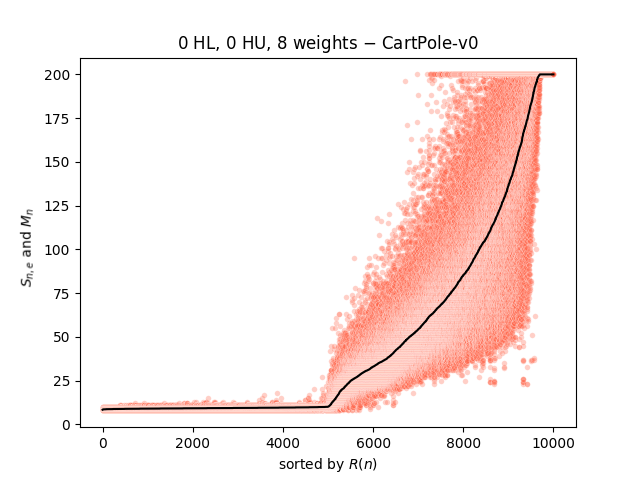
\includegraphics[width=.3\linewidth]{NN/CartPole_NN_HL_0_HU_0_scatter_score.png}
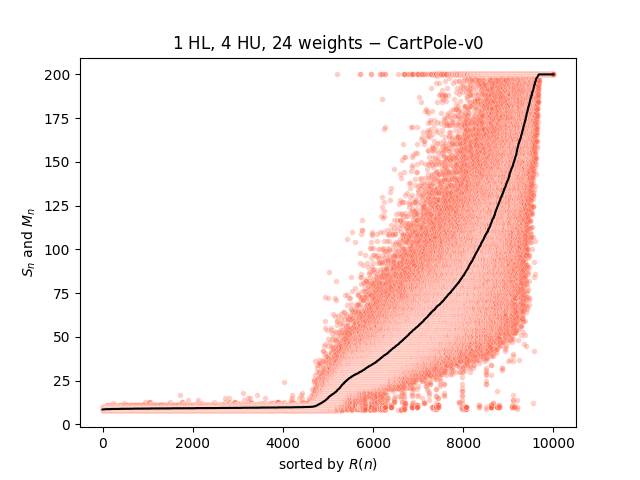
\includegraphics[width=.3\linewidth]{NN/CartPole_NN_HL_1_HU_4_scatter_score.png}
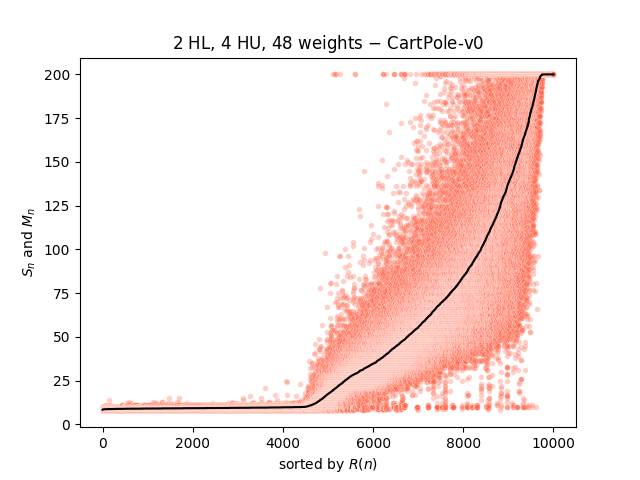
\includegraphics[width=.3\linewidth]{NN/CartPole_NN_HL_2_HU_4_scatter_score.png}}
\item \label{row:NN_Acrobot}  \raisebox{-0.5\height}{
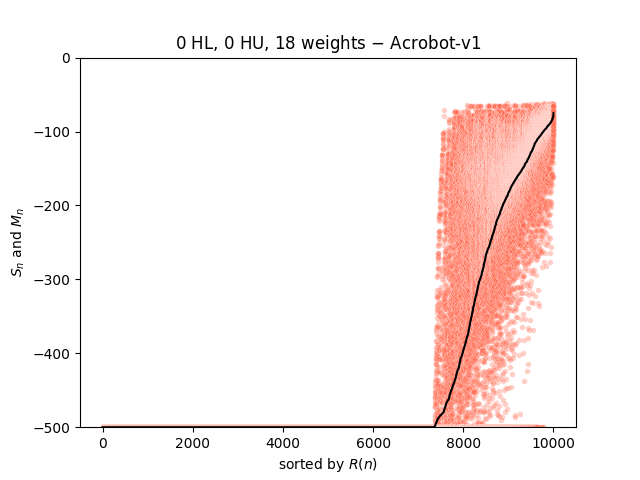
\includegraphics[width=.3\linewidth]{NN/Acrobot_NN_HL_0_HU_0_scatter_score.png}
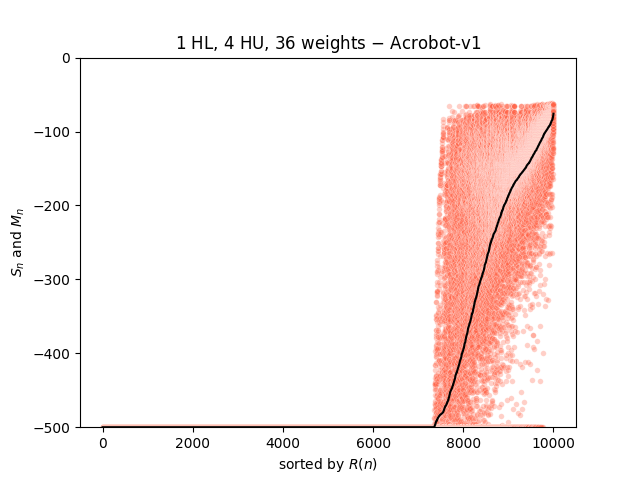
\includegraphics[width=.3\linewidth]{NN/Acrobot_NN_HL_1_HU_4_scatter_score.png}
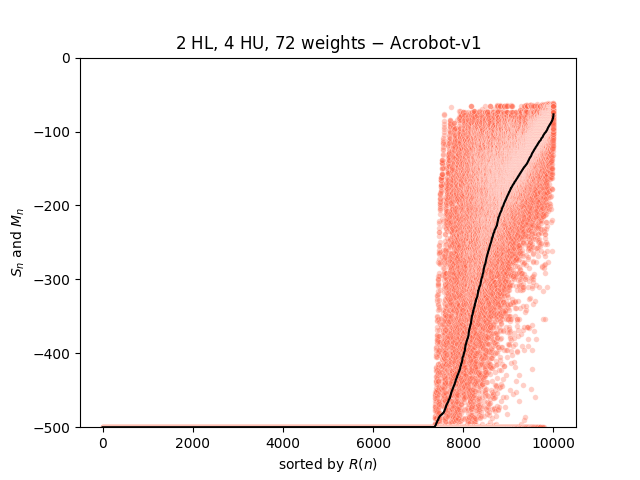
\includegraphics[width=.3\linewidth]{NN/Acrobot_NN_HL_2_HU_4_scatter_score.png}}
\item \label{row:NN_MountainCar}  \raisebox{-0.5\height}{
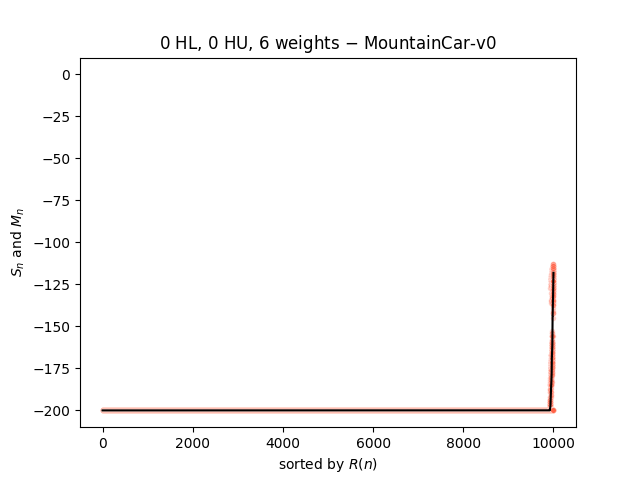
\includegraphics[width=.3\linewidth]{NN/MountainCar_NN_HL_0_HU_0_scatter_score.png}
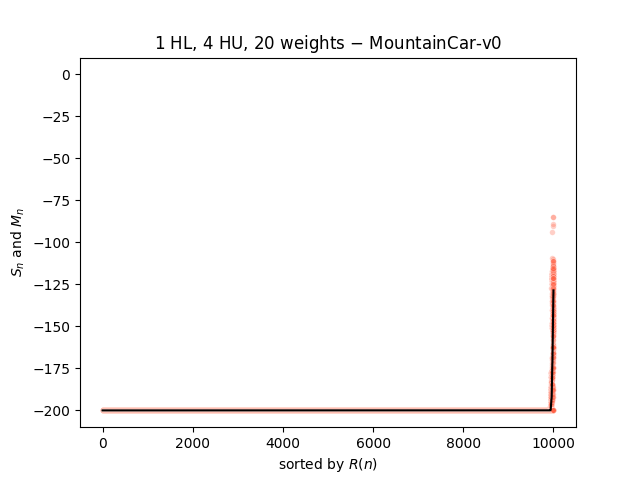
\includegraphics[width=.3\linewidth]{NN/MountainCar_NN_HL_1_HU_4_scatter_score.png}
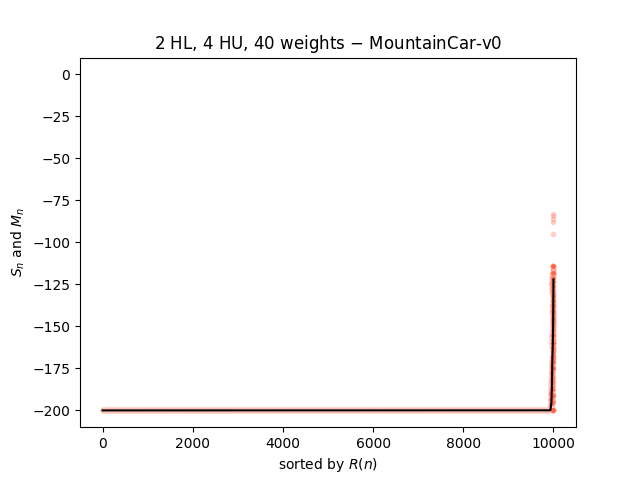
\includegraphics[width=.3\linewidth]{NN/MountainCar_NN_HL_2_HU_4_scatter_score.png}}
\item \label{row:NN_MountainCarCont}  \raisebox{-0.5\height}{
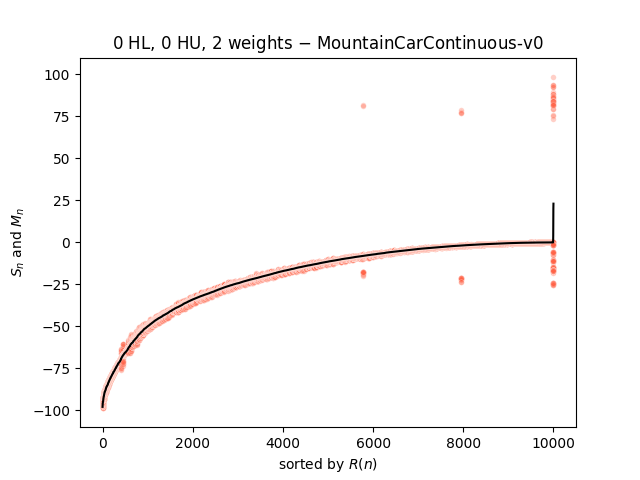
\includegraphics[width=.3\linewidth]{NN/MountainCarCont_NN_HL_0_HU_0_scatter_score.png}
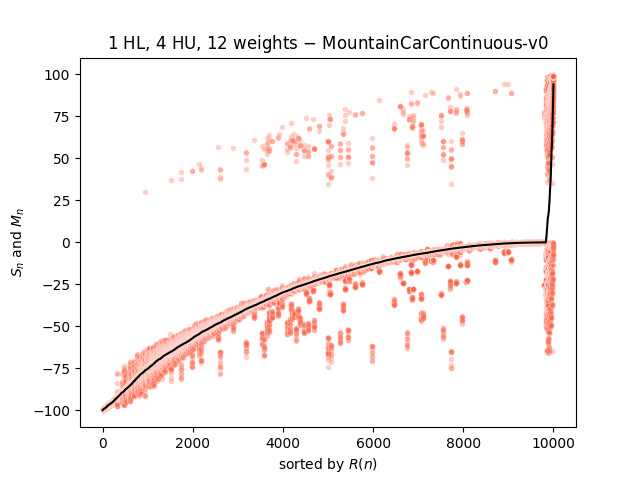
\includegraphics[width=.3\linewidth]{NN/MountainCarCont_NN_HL_1_HU_4_scatter_score.png}
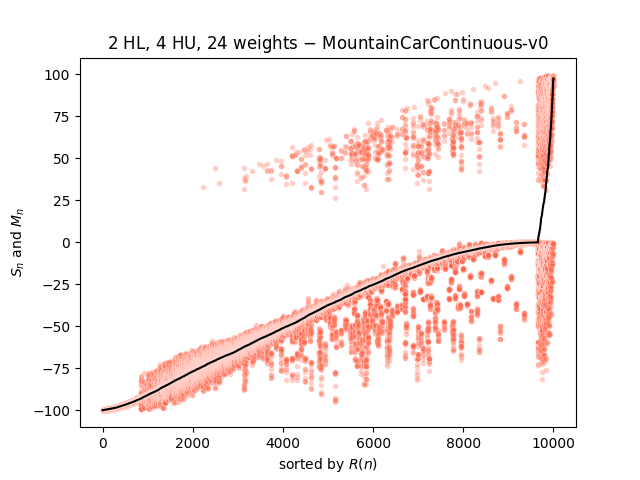
\includegraphics[width=.3\linewidth]{NN/MountainCarCont_NN_HL_2_HU_4_scatter_score.png}}
\item \label{row:NN_Pendulum}  \raisebox{-0.5\height}{
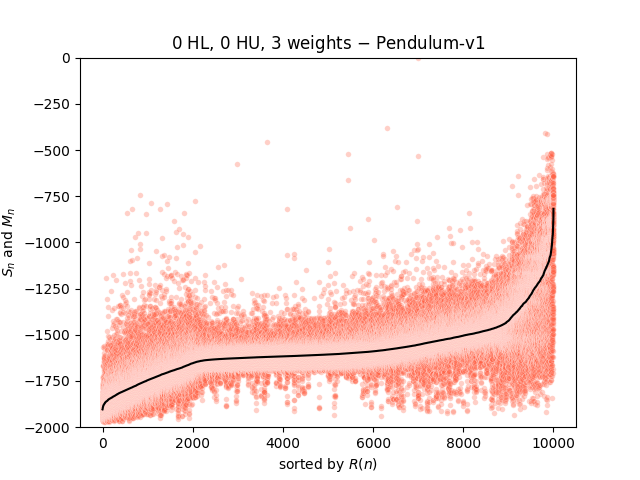
\includegraphics[width=.3\linewidth]{NN/Pendulum_NN_HL_0_HU_0_scatter_score.png}
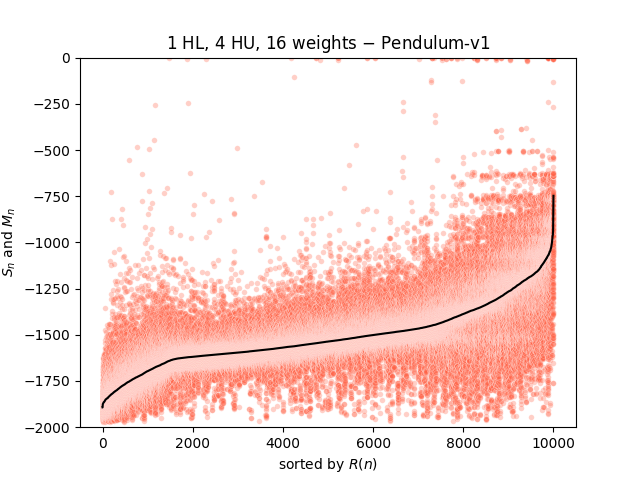
\includegraphics[width=.3\linewidth]{NN/Pendulum_NN_HL_1_HU_4_scatter_score.png}
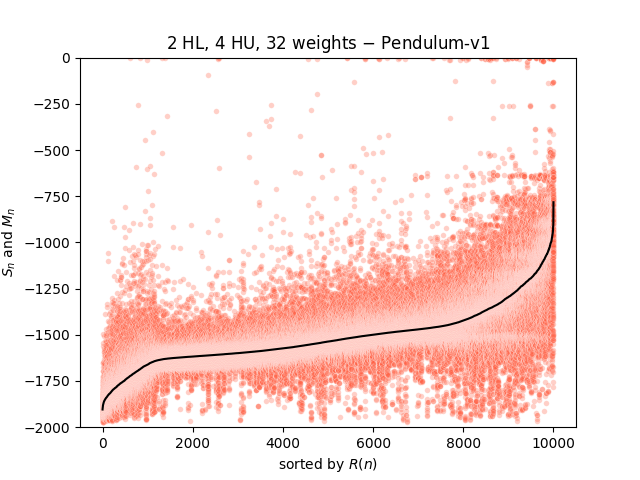
\includegraphics[width=.3\linewidth]{NN/Pendulum_NN_HL_2_HU_4_scatter_score.png}}
\end{figrow}
\caption[Results for the classic control environments using neural networks]{
  \textbf{Results for the classic control environments using neural networks.}
   Each row shows the results of one environment. The columns represent the different network architectures.
}
\label{fig:results_NN}
\end{figure}

\subsection{Polynomial Model}

\begin{figure}[!ht]
\begin{figrow}
\item \label{row:Polynomial_CartPole}  \raisebox{-0.5\height}{
\includegraphics[width=.3\linewidth]{experiment_1/without_bias/CartPole-v0_PolynomialNN_degree_1_scatter_score}
\includegraphics[width=.3\linewidth]{experiment_1/without_bias/CartPole-v0_PolynomialNN_degree_2_scatter_score}
\includegraphics[width=.3\linewidth]{experiment_1/without_bias/CartPole-v0_PolynomialNN_degree_3_scatter_score}}
\item \label{row:Polynomial_Acrobot}  \raisebox{-0.5\height}{
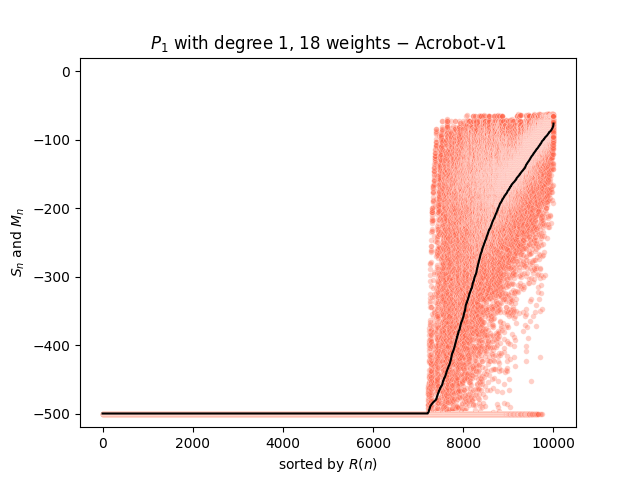
\includegraphics[width=.3\linewidth]{experiment_1/without_bias/Acrobot-v1_PolynomialNN_degree_1_scatter_score}
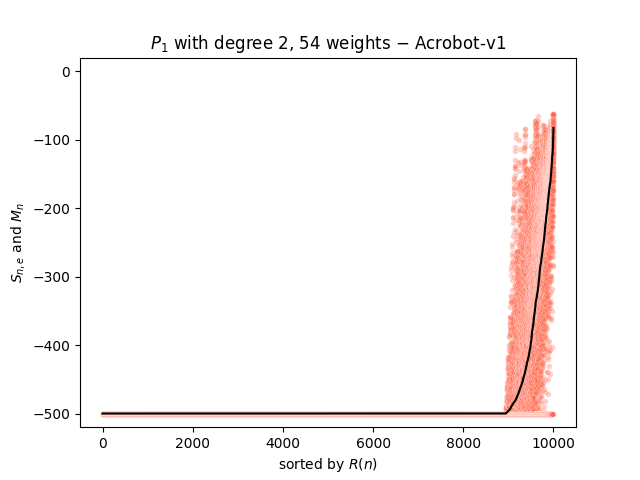
\includegraphics[width=.3\linewidth]{experiment_1/without_bias/Acrobot-v1_PolynomialNN_degree_2_scatter_score}
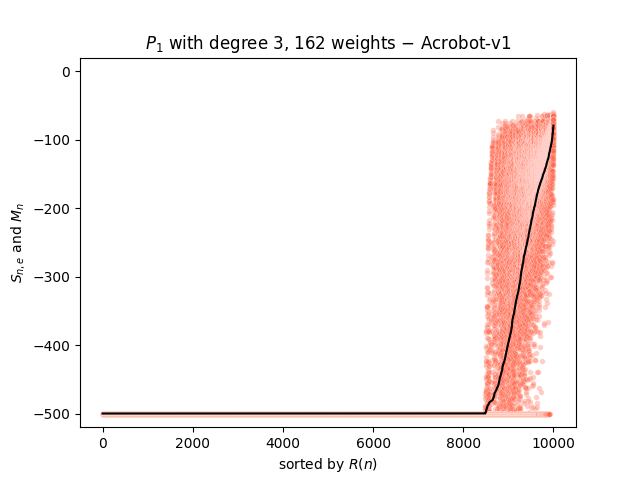
\includegraphics[width=.3\linewidth]{experiment_1/without_bias/Acrobot-v1_PolynomialNN_degree_3_scatter_score}}
\item \label{row:Polynomial_MountainCar}  \raisebox{-0.5\height}{
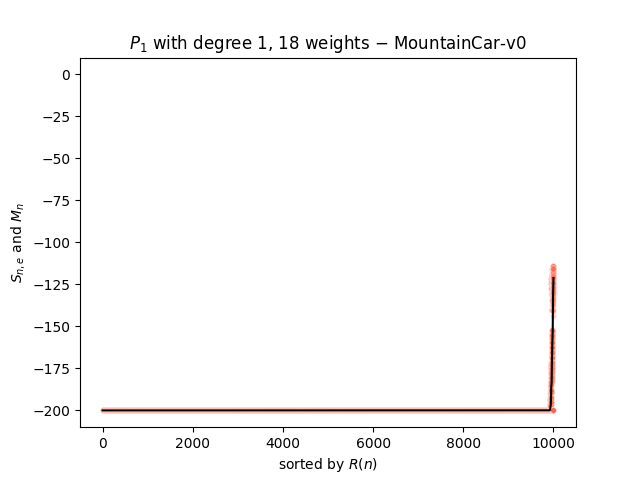
\includegraphics[width=.3\linewidth]{experiment_1/without_bias/MountainCar-v0_PolynomialNN_degree_1_scatter_score}
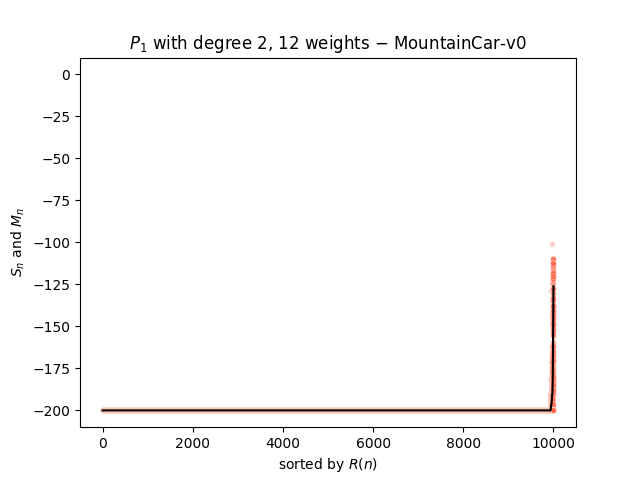
\includegraphics[width=.3\linewidth]{experiment_1/without_bias/MountainCar-v0_PolynomialNN_degree_2_scatter_score}
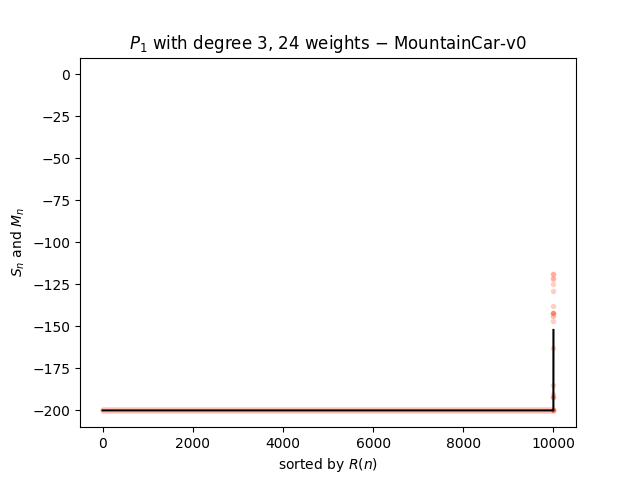
\includegraphics[width=.3\linewidth]{experiment_1/without_bias/MountainCar-v0_PolynomialNN_degree_3_scatter_score}}
\end{figrow}
\caption[Results for the classic control environments using polynomials]{
  \textbf{Results for the classic control environments using polynomials.}
   Each row shows the results of one environment. The columns represent the different degrees of the polynomials.
}
\label{fig:results_Polynomial}
\end{figure}

\begin{figure}[!ht]
\begin{figrow}
\item \label{row:Polynomial_CartPole_bias}  \raisebox{-0.5\height}{
\includegraphics[width=.3\linewidth]{experiment_1/with_bias/CartPole-v0_PolynomialNN_degree_1_scatter_score}
\includegraphics[width=.3\linewidth]{experiment_1/with_bias/CartPole-v0_PolynomialNN_degree_2_scatter_score}
\includegraphics[width=.3\linewidth]{experiment_1/with_bias/CartPole-v0_PolynomialNN_degree_3_scatter_score}}
\end{figrow}
\caption[Results for the classic control environments using polynomials with bias]{
  \textbf{Results for the classic control environments using polynomials with bias.}
   Each row shows the results of one environment. The columns represent the different degrees of the polynomials.
}
\label{fig:results_Polynomial_bias}
\end{figure}

Figure~\ref{fig:experiment_1_polynomial} shows the results of the first experiment for the two architectures of the polynomial model $P_1$ and $P_2$. I visualized the results of each model with bias connection in row (a) and without bias connection in row (b). The structure of the plots is identical for better comparison. The samples are ranked according to their mean score and aligned on the $x-$axis according to their rank. The scatter plots show all scores of the samples, whereas the lineplot illustrates the mean of each sample over all episodes.
Subfigure~\ref{fig:results_p1} shows the results of the polynomial model $P_1$ and Subfigure~\ref{fig:results_p2} shows the results of the polynomial model $P_2$.
\begin{figure}[!ht]
\begin{subfigure}{\textwidth}
\begin{figrow}
\item \label{row:P1_with_bias} \raisebox{-0.5\height}{
\includegraphics[width=.3\linewidth]{experiment_1/with_bias/PolynomialNN_degree_1_scatter_score.png}
\includegraphics[width=.3\linewidth]{experiment_1/with_bias/PolynomialNN_degree_2_scatter_score.png}
\includegraphics[width=.3\linewidth]{experiment_1/with_bias/PolynomialNN_degree_3_scatter_score.png}}
\item \label{row:P1_without_bias}  \raisebox{-0.5\height}{
\includegraphics[width=.3\linewidth]{experiment_1/without_bias/PolynomialNN_degree_1_scatter_score.png}
\includegraphics[width=.3\linewidth]{experiment_1/without_bias/PolynomialNN_degree_2_scatter_score.png}
\includegraphics[width=.3\linewidth]{experiment_1/without_bias/PolynomialNN_degree_3_scatter_score.png}}
\end{figrow}
\vspace*{-5mm}
\caption{Results of $P_1$ with bias (a) and without bias (b)}
\label{fig:results_p1}
\end{subfigure}
\begin{subfigure}{\textwidth}
\begin{figrow}
\item \label{row:P2_with_bias} \raisebox{-0.5\height}{
\includegraphics[width=.3\linewidth]{experiment_1/with_bias/Polynomial_degree_1_scatter_score.png}
\includegraphics[width=.3\linewidth]{experiment_1/with_bias/Polynomial_degree_2_scatter_score.png}
\includegraphics[width=.3\linewidth]{experiment_1/with_bias/Polynomial_degree_3_scatter_score.png}}
\item \label{row:P2_without_bias}  \raisebox{-0.5\height}{
\includegraphics[width=.3\linewidth]{experiment_1/without_bias/Polynomial_degree_1_scatter_score.png}
\includegraphics[width=.3\linewidth]{experiment_1/without_bias/Polynomial_degree_2_scatter_score.png}
\includegraphics[width=.3\linewidth]{experiment_1/without_bias/Polynomial_degree_3_scatter_score.png}}
\end{figrow}
\vspace*{-5mm}
\caption{Results of $P_2$ with bias (a) and without bias (b)}
\label{fig:results_p2}
\end{subfigure}
\caption[Results of experiment 1: polynomial models]{
  \textbf{Results of experiment 1: polynomial models.}
   The figures show the results of the first experiment with the two polynomial models. On the $x-$axis, we have the rank of each sample. On the $y-$axis, we have the scores of all samples and the mean as a lineplot. Each subplot shows the performance of the model with bias in row (a) and without bias in row (b). As we can see, both models perform equally good or bad. However, there is a huge difference in performance whether we are working with or without bias. In addition, we can see a difference in the slope of the mean values between polynomials with degree 1 and one with a higher degree.
}
\label{fig:experiment_1_polynomial}
\end{figure}
As we can see in the images, the plots of the two models almost look identical. Both models performed equally good or bad despite their different architecture and the different number of weights. Because of this similarity, I will not go into each model independently but instead discuss further results for both of them.

Looking at the linear model without bias, we can see a striking resemblance to the performance of the neural network previously shown in Section~\ref{ssec:benchmarks}. Looking further at the linear model, we can see that the curve of the mean score stays low until around $5'000$ but then goes up relatively steeply. That means that the linear model fails around 50\% to correctly guess the action. However, after that, we have a high probability to achieve a good score or even solve the task entirely during multiple episodes. There are also quite a few samples that could solve the task each time, indicated by the short straight black line at the top of the plot. Looking at the polynomials with degree 2, we can see that the scores increase already at around $2'000$, but the slope is less steep than for the linear model. In addition, there are fewer samples that could solve the task for each episode than there are for the linear model. Furthermore, the variance is higher for the polynomials with a higher degree compared to the linear model. If we look at the results of the polynomials with degree three, we can see that there is only a small boost compared to the polynomials of degree 2. The scores are overall slightly higher, but the slope is very similar to before. There is only a little difference between the two models even though the weights are doubled for $P_1$ and a half more for $P_2$. The large difference lies between the polynomials with degree 1 and polynomials with degree 2, respectively, degree 3. It seems that the complexity of the model depends more on the architecture of the model than on the number of weights.

In conclusion, with the linear model, we have a $50 \%$ chance of failing but the probability of actually solving the task for all episodes is higher than for the polynomials with a higher degree. That means that with the linear model, we have a larger fraction of samples that can solve the environment independent of the initialization conditions. At first glance, we could assume that this is an important aspect for such a model and choose the polynomial with degree 1 over one with a higher degree. However, we should remind ourselves that these experiments are rather unusual for an application since there is no learning involved and the number of samples is huge. In a common application, we would use some kind of training and want the model to sequentially improve its performance. Considering this aspect, when using a learning algorithm, we would not prefer the polynomials with degree 1 as we might get stuck in a fitness plateau when the algorithm has no method of dealing with this behavior.

Another observation we can make from Figure~\ref{fig:experiment_1_polynomial} is that the bias influences the performance of the model significantly. We already saw this behavior with the neural network in Section~\ref{ssec:benchmarks}. Thus, the influence of the bias is not specific to neural networks but seems to be more of a general factor.

\todo[inline]{Restrukturing this section, adjust text to new plots}

\subsection{Binary Tree Model}
For the binary trees, I tested three models, one with 1 node, one with 4 nodes, and one with 8 nodes. Since the previous experiments suggest that using bias has a negative effect, the following experiments do not include bias. Figure~\ref{fig:results_BinaryTree} shows the results for all five classic control environments with the binary tree models.
\begin{figure}[!ht]
\begin{figrow}
\item \label{row:BinaryTree_CartPole} \raisebox{-0.5\height}{
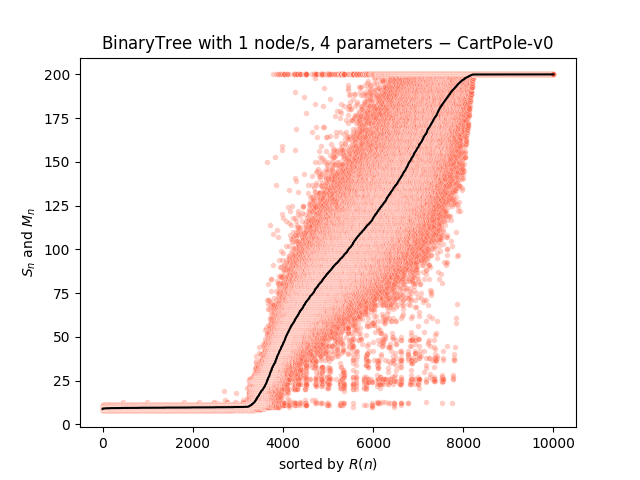
\includegraphics[width=.3\linewidth]{Binary_Tree/CartPole_BinaryTree_1_nodes_scatter_score.png}
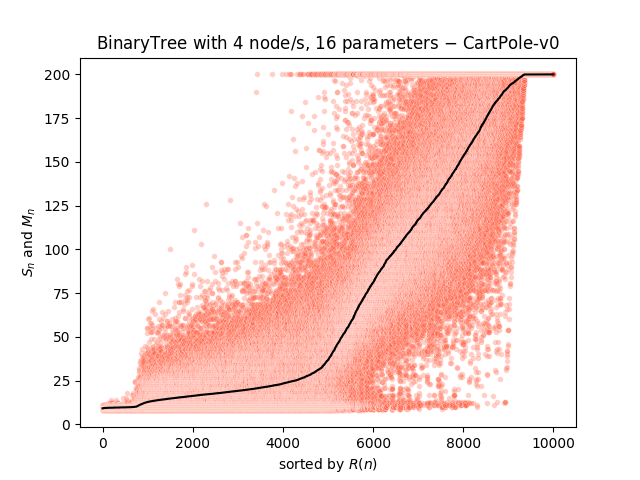
\includegraphics[width=.3\linewidth]{Binary_Tree/CartPole_BinaryTree_4_nodes_scatter_score.png}
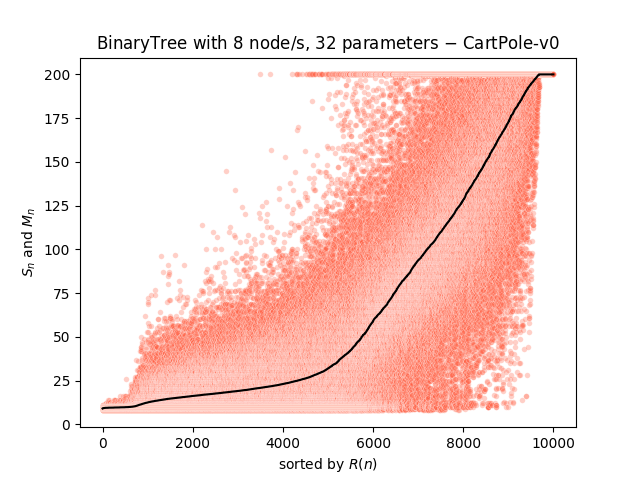
\includegraphics[width=.3\linewidth]{Binary_Tree/CartPole_BinaryTree_8_nodes_scatter_score.png}}
\item \label{row:BinaryTree_Acrobot} \raisebox{-0.5\height}{
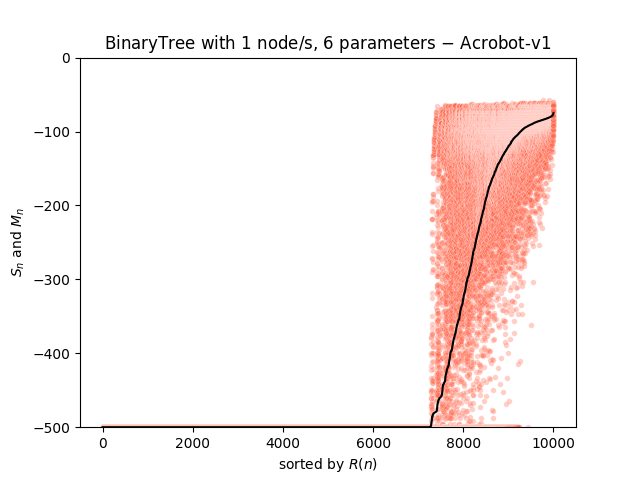
\includegraphics[width=.3\linewidth]{Binary_Tree/Acrobot_BinaryTree_1_nodes_scatter_score.png}
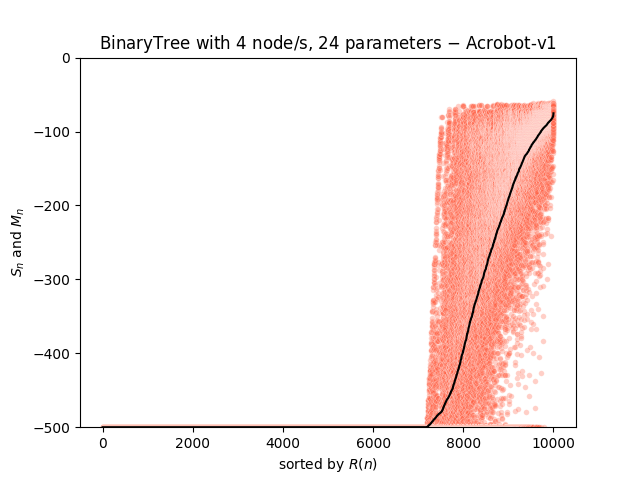
\includegraphics[width=.3\linewidth]{Binary_Tree/Acrobot_BinaryTree_4_nodes_scatter_score.png}
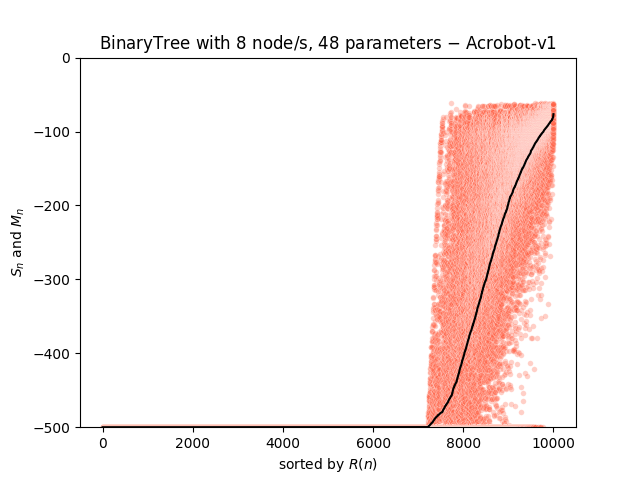
\includegraphics[width=.3\linewidth]{Binary_Tree/Acrobot_BinaryTree_8_nodes_scatter_score.png}}
\item \label{row:BinaryTree_MountainCar} \raisebox{-0.5\height}{
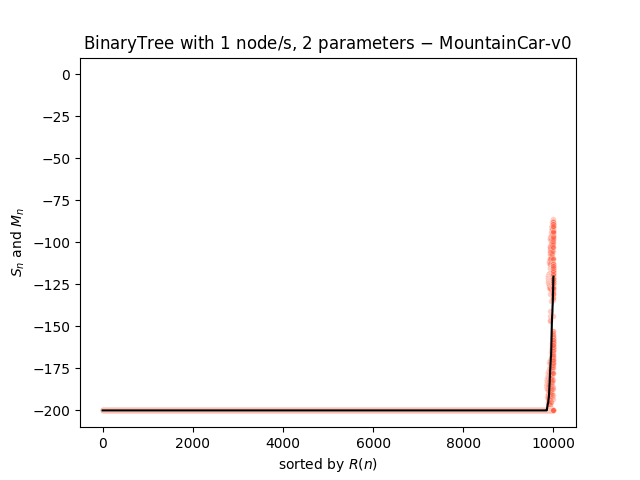
\includegraphics[width=.3\linewidth]{Binary_Tree/MountainCar_BinaryTree_1_nodes_scatter_score.png}
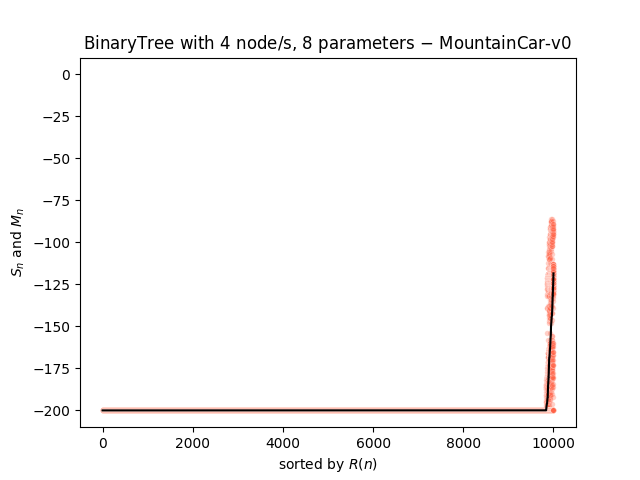
\includegraphics[width=.3\linewidth]{Binary_Tree/MountainCar_BinaryTree_4_nodes_scatter_score.png}
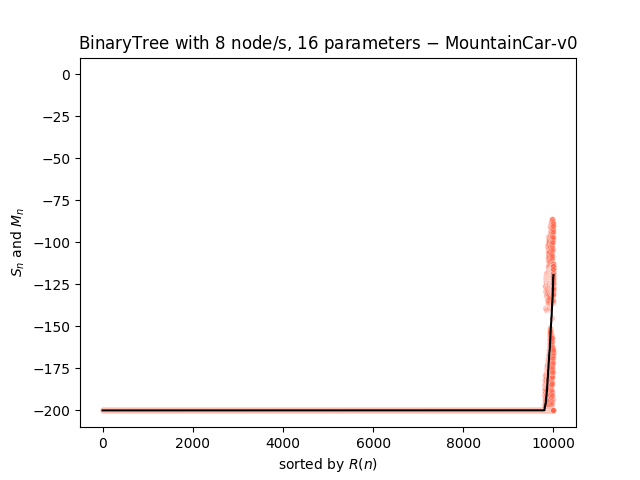
\includegraphics[width=.3\linewidth]{Binary_Tree/MountainCar_BinaryTree_8_nodes_scatter_score.png}}
\item \label{row:BinaryTree_MountainCarCont}  \raisebox{-0.5\height}{
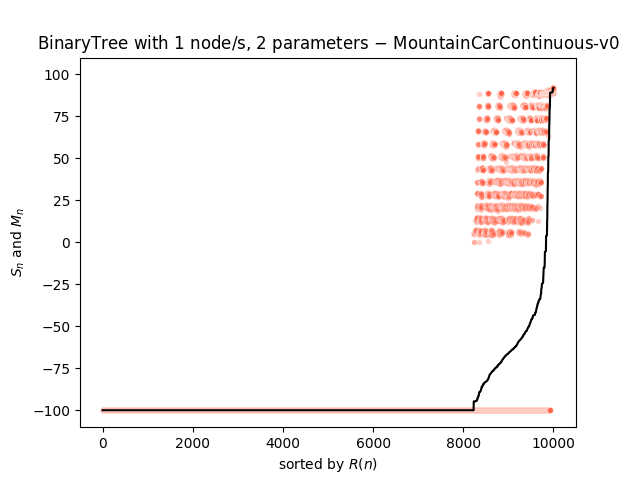
\includegraphics[width=.3\linewidth]{Binary_Tree/MountainCarCont_BinaryTree_1_nodes_scatter_score.png}
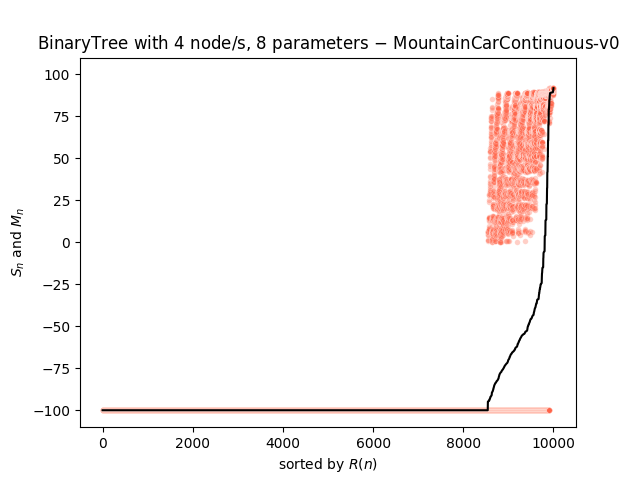
\includegraphics[width=.3\linewidth]{Binary_Tree/MountainCarCont_BinaryTree_4_nodes_scatter_score.png}
\includegraphics[width=.3\linewidth]{Binary_Tree/MountainCarCont_BinaryTree_8_nodes_scatter_score.png}}
\item \label{row:BinaryTree_Pendulum} \raisebox{-0.5\height}{
\includegraphics[width=.3\linewidth]{Binary_Tree/Pendulum_BinaryTree_1_nodes_scatter_score.png}
\includegraphics[width=.3\linewidth]{Binary_Tree/Pendulum_BinaryTree_4_nodes_scatter_score.png}
\includegraphics[width=.3\linewidth]{Binary_Tree/Pendulum_BinaryTree_8_nodes_scatter_score.png}}
\end{figrow}
\caption[Results for the classic control environments using binary trees]{
  \textbf{Results for the classic control environments using binary trees.}
   Each row shows the results of one environment. The columns represent the different configurations for the binary tree models.
}
\label{fig:results_BinaryTree}
\end{figure}

Comparing the results using binary trees with the ones using neural networks shown in Figure~\ref{fig:results_NN}, we can see a few differences. For the environment \verb|CartPole|, we can see that we reach overall better scores with the binary trees. Comparing the neural network without hidden layers with the binary tree with only one node, we have a similar curve, but the lineplot representing the mean scores sets off much earlier at around 3'500 for the binary tree than the one for the neural network, which sets off at around 5'000. In addition, the binary tree has a higher chance of reaching a maximal mean score, indicated by the straight black line at the top right. For the more complex architectures, it gets more interesting. The binary tree with four nodes can already raise the mean value under 1'000 samples. That tells us that the problem of having a fitness plateau is reduced a lot. Thus, when using a learning algorithm, the binary tree has a better chance of solving the problem without getting stuck in a fitness plateau. The chance of reaching a maximal mean score decreases with adding more nodes to the binary tree. That could be caused by the increasing complexity of the binary tree, which makes it harder to guess the weights correctly. Furthermore, the scores are more spread out for the binary trees than for the neural networks. That results in a higher variance for the binary tree.

For the environment \verb|Acrobot|, the plots do not show a major difference between the two models. Overall, we can say that both models reach similar scores and mean values. However, the scores seem to be more spread out for the binary trees than for the neural networks, indicating a higher variance.

The \verb|MountainCar| environment is difficult for a learning algorithm because of the large fitness plateau we can see in the plots. Comparing the two models, binary trees and neural networks, we can see that the binary trees are more likely to reach a better score. However, there is still a large risk to land on a fitness plateau. In addition, the scores are spread wider for the binary tree than for the neural network. That indicates a higher variance.

The results for the environment \verb|MountainCarContinuous| look very different for the binary trees than for the neural networks. Neural networks show an increasing line for the mean scores. The binary trees have a lot of low performers. However, there are a few samples that are able to reach a positive score. The neural network without hidden layers could not reach these high mean scores.

For the \verb|Pendulum| environment, we can see that the binary trees perform increasingly better with more nodes. The difference between the two models, neural networks and binary trees is not huge. However, we can see that using neural networks results in a few higher mean scores. But with the binary trees we have a slightly higher score in the middle area. In addition, the binary trees show a higher variance than the neural networks.
\todo[inline]{Improve text}

\subsection{Bias Investigation}
In their paper, \cite{oller_analyzing_2020} mentioned that we are more likely to have top performers when dropping bias connections. Figure~\ref{fig:results_NN_bias} shows the results without using bias.
\begin{figure}[!ht]
\begin{figrow}
\item \label{row:NN_with_bias_CartPole} \raisebox{-0.5\height}{
\includegraphics[width=.3\linewidth]{experiment_2/default/with_bias/CartPole-v0_NN_HL_0_HU_0_scatter_score}
\includegraphics[width=.3\linewidth]{experiment_2/default/with_bias/CartPole-v0_NN_HL_1_HU_4_scatter_score}
\includegraphics[width=.3\linewidth]{experiment_2/default/with_bias/CartPole-v0_NN_HL_2_HU_4_scatter_score}}
\item \label{row:NN_with_bias_Pendulum} \raisebox{-0.5\height}{
\includegraphics[width=.3\linewidth]{experiment_2/default/with_bias/MountainCar-v0_NN_HL_0_HU_0_scatter_score}
\includegraphics[width=.3\linewidth]{experiment_2/default/with_bias/MountainCar-v0_NN_HL_1_HU_4_scatter_score}
\includegraphics[width=.3\linewidth]{experiment_2/default/with_bias/MountainCar-v0_NN_HL_2_HU_4_scatter_score}}
\item \label{row:NN_with_bias_Pendulum} \raisebox{-0.5\height}{
\includegraphics[width=.3\linewidth]{experiment_2/default/with_bias/Pendulum-v1_NN_HL_0_HU_0_scatter_score}
\includegraphics[width=.3\linewidth]{experiment_2/default/with_bias/Pendulum-v1_NN_HL_1_HU_4_scatter_score}
\includegraphics[width=.3\linewidth]{experiment_2/default/with_bias/Pendulum-v1_NN_HL_2_HU_4_scatter_score}}
\end{figrow}
\caption[Results using neural networks without bias]{
  \textbf{Results using neural networks without bias.}
   The plots show the results of the classic control environments using neural networks without bias.
}
\label{fig:results_NN_bias}
\end{figure}
Comparing these plots with the ones without using bias in Figure~\ref{fig:results_NN}, we can see the negative impact the bias has on the effectiveness of the model. The scores are overall lower and get even worse with the increased complexity of the model. Therefore, we can confirm the interesting observation of the authors, namely, that using bias is counterproductive in this experimental setting.

Figure~\ref{fig:results_NN_weights} shows the results of tripling the number of weights for each network architecture. Row (a) shows the results using bias, and row (b) shows the results without bias for the \verb|CartPole| environment.
\begin{figure}[!ht]
\begin{figrow}
\item \label{row:NN_with_bias_wfactor_3} \raisebox{-0.5\height}{
\includegraphics[width=.3\linewidth]{experiment_2/weights/weight_factor_3/with_bias/HL_0_HU_0_scatter_score.png}
\includegraphics[width=.3\linewidth]{experiment_2/weights/weight_factor_3/with_bias/HL_1_HU_4_scatter_score.png}
\includegraphics[width=.3\linewidth]{experiment_2/weights/weight_factor_3/with_bias/HL_2_HU_4_scatter_score.png}}
\item \label{row:NN_without_bias_wfactor_3}  \raisebox{-0.5\height}{
\includegraphics[width=.3\linewidth]{experiment_2/weights/weight_factor_3/without_bias/HL_0_HU_0_scatter_score.png}
\includegraphics[width=.3\linewidth]{experiment_2/weights/weight_factor_3/without_bias/HL_1_HU_4_scatter_score.png}
\includegraphics[width=.3\linewidth]{experiment_2/weights/weight_factor_3/without_bias/HL_2_HU_4_scatter_score.png}}
\end{figrow}
\vspace*{-5mm}
\caption[Results of experiment 2: weights]{
  \textbf{Results of experiment 2: weights.}
   The figure shows the results of tripling the number of weights for the three neural network architectures for one classic control environment. Row (a) shows the results with bias connections, and row (b) shows the results without bias connections. Despite the increased number of weights, there is no visible difference in the plots compared to the ones shown in Figure~\ref{fig:results_NN} and Figure~\ref{fig:results_NN_bias}.
}
\label{fig:results_NN_weights}
\end{figure}
Comparing the plots of row (a) from Figure~\ref{fig:results_NN_weights} with the ones in Figure~\ref{fig:results_NN_bias}, we can barely see a difference. The slope of the mean values looks the same. The data points do not show different behavior. The same applies to comparing row (b) from Figure~\ref{fig:results_NN_weights} to Figure~\ref{fig:results_NN}. Thus, we can conclude that increasing the number of weights does not impact the achieved score of the model significantly. In addition, the same experiment with the polynomial models $P_1$ and $P_2$ draws the same conclusion.

Figure~\ref{fig:experiment_2_layers} shows the results of altering the number of layers in a network. For the networks with bias connections, the performance gets significantly worse with an increased number of layers. The networks without bias connections seem to be more robust. Still, the steepness of the slope of the line plots decreases with an increased number of layers.
\begin{figure}[!ht]
\begin{figrow}
\item \label{row:NN_with_bias_layers} \raisebox{-0.5\height}{
\includegraphics[width=.3\linewidth]{experiment_2/layers/with_bias/HL_4_scatter_score.png}
\includegraphics[width=.3\linewidth]{experiment_2/layers/with_bias/HL_6_scatter_score.png}
\includegraphics[width=.3\linewidth]{experiment_2/layers/with_bias/HL_8_scatter_score.png}}
\item \label{row:NN_without_layers}  \raisebox{-0.5\height}{
\includegraphics[width=.3\linewidth]{experiment_2/layers/without_bias/HL_4_scatter_score.png}
\includegraphics[width=.3\linewidth]{experiment_2/layers/without_bias/HL_6_scatter_score.png}
\includegraphics[width=.3\linewidth]{experiment_2/layers/without_bias/HL_8_scatter_score.png}}
\end{figrow}
\caption[Results of experiment 2: layers]{
  \textbf{Results of experiment 2: layers.}
   The plots show the result of increasing the number of hidden layers gradually. Again, row (a) represents the networks with bias connections, row (b) the ones without bias connections. As we can see, the results in row (a) get worse with an increase in the number of layers. Row (b) is less extreme but there is also a loss of steepness with an increasing number of hidden layers.
}
\label{fig:experiment_2_layers}
\end{figure}

Figure~\ref{fig:experiment_2_neurons} shows the results of increasing the number of neurons in each hidden layer for a network with two hidden layers. Comparing the plots with the ones in Figure~\ref{fig:experiment_2_default}, we can see a slight improvement in the plots without bias connections in rows (a). In addition, the data points seem to be more spread out, indicating a higher variance. The results of the networks without using bias connections do not show much difference. The slope is a little less steep with increased neurons.
\begin{figure}[!ht]
\begin{figrow}
\item \label{row:NN_with_bias_neurons} \raisebox{-0.5\height}{
\includegraphics[width=.3\linewidth]{experiment_2/neurons/with_bias/HL_2_HU_5_scatter_score.png}
\includegraphics[width=.3\linewidth]{experiment_2/neurons/with_bias/HL_2_HU_8_scatter_score.png}
\includegraphics[width=.3\linewidth]{experiment_2/neurons/with_bias/HL_2_HU_10_scatter_score.png}}
\item \label{row:NN_without_neurons}  \raisebox{-0.5\height}{
\includegraphics[width=.3\linewidth]{experiment_2/neurons/without_bias/HL_2_HU_5_scatter_score.png}
\includegraphics[width=.3\linewidth]{experiment_2/neurons/without_bias/HL_2_HU_8_scatter_score.png}
\includegraphics[width=.3\linewidth]{experiment_2/neurons/without_bias/HL_2_HU_10_scatter_score.png}}
\end{figrow}
\caption[Results of experiment 2: neurons]{
  \textbf{Results of experiment 2: neurons.}
  The plots show the result of increasing the number of neurons for each layer in a network with two hidden layers. The plots in row (a) represent the networks with bias connections, the ones in row (b) represent the networks without bias connections. We can see a slight improvement in row (a).
}
\label{fig:experiment_2_neurons}
\end{figure}

\todo[inline]{Restructuring, adjust text}

\section{Discussion}
This chapter delivered a direct comparison between neural networks and alternative models like polynomials and binary trees. In addition, I investigated the impact of bias in these settings. I was able to show that binary tree models can compare with neural networks in solving the classic control environment.

\todo[inline]{Explain more. Include here or just conclusion?}
